%Everything is owned by Aditya Teraiya. Unauthorized use is prohibited.
\documentclass[11pt, a4paper]{article}
\usepackage[utf8]{inputenc}
\usepackage[margin=1in, top=1.3in]{geometry} % Adjusted top margin 
% --- Core Layout & Structure ---
\usepackage{fancyhdr, titlesec, multicol}

% --- Advanced Mathematics ---
\usepackage{amsmath, amssymb, amsfonts, mathtools}

% --- Graphics, Colors & Custom Boxes ---
\usepackage{graphicx, xcolor, tcolorbox, tikz}
\usetikzlibrary{shapes.geometric,shapes.arrows,calc,shapes.symbols}
\tikzstyle{startstop} = [rectangle, rounded corners, minimum width=3cm, minimum height=1cm,text centered, draw=black, fill=red!10]
\tikzstyle{io} = [trapezium, trapezium left angle=70, trapezium right angle=110, minimum width=3cm, minimum height=1cm, text centered, draw=black, fill=blue!30]
%\tikzstyle{loop} = [hexagon, hexagon left angle=60, hexagon right angle=60, minimum width=3cm, minimum height=1cm, text centered, draw=black, fill=yellow!30]
\tikzset{
  hexagon/.style={
    signal,
    signal to=east and west, % This creates the /---\ \---/ points on both sides
    signal pointer angle=120, % Controls the "pointiness" (default is 90)
    draw,
    minimum width=2cm, 
    minimum height=1cm, 
    fill=purple!50
  }
}
\tikzstyle{process} = [rectangle, minimum width=3cm, minimum height=1cm, text centered, draw=black, fill=orange!30]
\tikzstyle{decision} = [diamond, minimum width=3cm, minimum height=1cm, text centered, draw=black, fill=green!30]
\tikzstyle{loop}=[hexagon, minimum width=3cm, minimum height=1cm, text centered, draw=black, fill=purple!30]
\tikzstyle{arrow} = [thick,->,>=stealth]


% --- Text Formatting & Lists ---
\usepackage{enumitem, url, hyperref}
\usepackage{bookmark}

% --- Tables, Figures & Captions ---
\usepackage{booktabs, array, float, caption, subcaption}

% --- Code Snippets & Citations ---
\usepackage{lipsum, listings}

\lstdefinestyle{codestyle}{
  language=C,
  basicstyle=\ttfamily\footnotesize,
  keywordstyle=\color{blue},
  commentstyle=\color{green!50!black},
  stringstyle=\color{red!60!black},
  numbers=left,
  numberstyle=\tiny\color{gray},
  stepnumber=1,
  showstringspaces=false,
  breaklines=true,
  frame=single,
  backgroundcolor=\color{gray!5},
  rulecolor=\color{gray!30},
  columns=fullflexible,
  keepspaces=true
}

\lstset{style=codestyle}

% Custom Box Definition as requested
\newtcolorbox{box1}{
  colback=purple!10!white,
  colframe=purple!75!black,
  boxrule=0pt,
  leftrule=3pt,
  rightrule=0pt,
  toprule=0pt,
  bottomrule=0pt,
  sharp corners,
  left=4pt,right=4pt,top=4pt,bottom=4pt
}

\newtcolorbox{box2}{
  colback=blue!10!white,
  colframe=blue!75!black,
  boxrule=0pt,
  leftrule=3pt,
  rightrule=0pt,
  toprule=0pt,
  bottomrule=0pt,
  sharp corners,
  left=4pt,right=4pt,top=4pt,bottom=4pt
}

% Header Layout Configuration
\pagestyle{fancy}
\fancyhf{} % Clear default header and footer settings
\renewcommand{\headrulewidth}{0.5pt} % Adds a neat horizontal divider under your header metadata

% Top Left Margin Content
\fancyhead[L]{%
  \textcolor{blue}{\textbf{\href{https://github.com/adi42wastaken}{Aditya Teraiya}}} \\
  \textcolor{cyan}{\textbf{\href{mailto: bmat2546@isibang.ac.in}{bmat2546}}} \\
   Indian Statistical Institute, Bangalore.
}

% Top Right Margin Content
\fancyhead[R]{%
  \textbf{Subject:} Fundamentals of Comptuing and programing \\
  \textbf{Assignment} \#1 \\
  \textbf{Date:} \today
}

% Increase header height so the three rows of text do not collide with the page boundaries
\setlength{\headheight}{42pt}

\begin{document}
\section{Theorical questions}
\begin{enumerate}
  \item Explain the characteristics and importance of algorithms.\\
  \begin{enumerate}
  \item Finiteness: The algorithm must always terminate after a finite number of steps. It cannot loop infinitely.

\item Definiteness: Each step must be rigorously and unambiguously defined. There is no room for interpretation (e.g., "add a small number" is invalid; "add 1" is definite).

\item Input: It takes zero or more defined inputs (initial quantities provided before execution begins).

\item Output: It produces at least one output (the result that has a specified relation to the inputs).

\item Effectiveness: Every operation must be basic enough that it could, in principle, be carried out exactly and in a finite amount of time using just pen and paper.
  \end{enumerate}
   Algorithms are important as they provide a standardized, language-agnostic way to solve problems efficiently.
  \item Distinguish between algorithms, flowcharts, pseudocode, and programs.
  \begin{enumerate}
    \item Algorithm: The abstract logical concept or method.
    \item Flowchart: A text-based, structured draft of the algorithm.
    \item Pseudocode: A graphical representation of the algorithm's topology.
    \item Programs: The concrete implementation written for a machine.
  \end{enumerate}
  \item Discuss various symbols with labeled diagrams.
  \begin{enumerate}
    \item Start/Stop: Marks the absolute Start and End points of the algorithm. Every flowchart must begin and terminate with this symbol.
    \item Input/Output: Represents data entering the system or leaving the system.
    \item Process: Represents an operational step, such as a mathematical calculation, variable assignment, or data manipulation.
    \item Decision: The branching point where the logic evaluates a condition. True and False
    \item Loop (hexagon): Represents the looping condition. It could be for loop, while loop or do-while loop.
    \item Flowlines (Arrows): The directional vectors that connect the symbols, establishing the strict chronological sequence of execution.
  \end{enumerate}
\end{enumerate}
\begin{tikzpicture}
    \node (s)[startstop]{Start/Stop};
    \node (i)[io, right of=s, xshift=3cm]{Input/Output};
    \node (p)[process, right of=i, xshift=3cm]{Process};
    \node (d)[decision, below of=s, yshift=-1cm]{Decision};
    \node (h)[hexagon, below of=i, yshift=-1cm]{Loop};
    \draw[->] ($(h)+(3,0)$)--($(p.south)+(-1,-1)$)--($(p.south)+(2,-1)$)--($(h.east)+(5,-1)$);
  \end{tikzpicture}
\section{Sequence type}
\begin{enumerate}
  \item Write an algorithm and draw the flowchart to find the area and perimeter of the circle
  \begin{enumerate}[label=\arabic*:]
    \item start
    \item read the radius $r$
    \item print the circumferance $2\pi r$ and area $\pi r^2$
    \item stop
  \end{enumerate}
  \begin{tikzpicture}[node distance=2cm]

\node (start) [startstop] {start};
\node (in1) [io, below of=start] {read r};
\node (out1) [io, below of=in1] {print $2\pi\cdot r$ , $\pi\cdot r^2$};
\node (stop) [startstop, below of=out1] {stop};
\draw [arrow] (start) -- (in1);
\draw [arrow] (in1) -- (out1);
\draw [arrow] (out1) -- (stop);

\end{tikzpicture}
  \item Write an algorithm and draw a flowchart to convert temperature from Celsius to
Fahrenheit. and vice versa
\begin{enumerate}[label=\arabic*:]
  \item start
  \item read the temperature in Celsius $C$
  \item print $F = \frac{9}{5}C + 32$
  \item stop
\end{enumerate}
 \begin{tikzpicture}[node distance=2cm]

\node (start) [startstop] {start};
\node (in1) [io, below of=start] {read C};
\node (out1) [io, below of=in1] {print $F = \frac{9}{5}C + 32$};
\node (stop) [startstop, below of=out1] {stop};
\draw [arrow] (start) -- (in1);
\draw [arrow] (in1) -- (out1);
\draw [arrow] (out1) -- (stop);

\end{tikzpicture}
\begin{enumerate}[label=\arabic*:]
  \item start
  \item read the temperature in Fahrenheit $F$
  \item print $C = \frac{5}{9}(F - 32)$
  \item stop
\end{enumerate}
 \begin{tikzpicture}[node distance=2cm]

\node (start) [startstop] {start};
\node (in1) [io, below of=start] {read F};
\node (out1) [io, below of=in1] {print $C = \frac{5}{9}(F - 32)$};
\node (stop) [startstop, below of=out1] {stop};
\draw [arrow] (start) -- (in1);
\draw [arrow] (in1) -- (out1);
\draw [arrow] (out1) -- (stop);

\end{tikzpicture}
 \item Write an algorithm and draw the flowchart to determine the Simple Interest, reading
Principle, Rate and Time.
\begin{enumerate}[label=\arabic*:]
  \item start
  \item read the Principle $P$, Rate $R$ and Time $T$, define the Simple Interest $SI$
  \item Process $SI = \frac{P \cdot R \cdot T}{100}$
  \item print $SI$
  \item stop
\end{enumerate}
\begin{tikzpicture}[node distance=2cm]
  \node (start)[startstop]{start};
  \node (in1)[io, below of=start]{read $P,R,T$ define $SI$};
  \node (pro1)[process, below of=in1]{Process $SI=\frac{P \cdot R \cdot T}{100}$};
  \node (ou2)[io, below of=pro1]{print $SI$};
  \node (stop)[startstop, below of=ou2]{stop};
  \draw [arrow] (start)--(in1)--(pro1)--(ou2)--(stop);
\end{tikzpicture}

 \item Write algorithms and flowcharts:
 \begin{enumerate}
  \item Using a third variable
  \begin{enumerate}[label=\arabic*:]
    \item start
    \item read a,b,c
    \item process c=a; a=b; b=c;
    \item print a,b
    \item stop
    \end{enumerate}
    \begin{tikzpicture}[node distance=2cm]
  \node (start)[startstop]{start};
  \node (in1)[io, below of=start]{read $a,b$ define $c$};
  \node (pro1)[process, below of=in1]{Process $c=a; a=b; b=c;$};
  \node (ou2)[io, below of=pro1]{print $a,b$};
  \node (stop)[startstop, below of=ou2]{stop};
  \draw [->] {(start)--(in1)--(pro1)--(ou2)--(stop)};
\end{tikzpicture}
  \item Without using a third variable
   \begin{enumerate}[label=\arabic*:]
    \item start
    \item read a,b
    \item process a=a+b;b=a-b;a=a-b;
    \item print a,b
    \item stop
    \end{enumerate}
    \begin{tikzpicture}[node distance=2cm]
  \node (start)[startstop]{start};
  \node (in1)[io, below of=start]{read $a,b$};
  \node (pro1)[process, below of=in1]{Process $a=a+b; b=a-b; a=a-b;$};
  \node (ou2)[io, below of=pro1]{print $a,b$};
  \node (stop)[startstop, below of=ou2]{stop};
  \draw [->] {(start)--(in1)--(pro1)--(ou2)--(stop)};
\end{tikzpicture}
\end{enumerate}
\end{enumerate}
\section{Conditional type}
\begin{enumerate}
  \item Write an algorithm and draw the flowchart to check whether number is even or odd.
    \begin{enumerate}[label=\arabic*:]
    \item start
    \item read $a$
    \item process if the remainder of $a$ when divided by 2 is 0
    \item print (if true) even; (if false) odd
    \item stop
    \end{enumerate}
    \begin{tikzpicture}[node distance=2cm]
      \node (start)[startstop]{start};
      \node (in1)[io, below of=start]{read $a$};
      \node (d1)[decision, below of=in1]{$a\% 2==0$};
      \node (ou1)[io, left of=d1, xshift=-3cm]{print Even};
      \node (ou2)[io, right of=d1, xshift=3cm]{print Odd};
      \node (stop)[startstop,below of=d1]{stop};
      \draw [->](start)--(in1);
      \draw [->](in1)--(d1);
      \draw [->](d1)--(ou1) node[midway, above] {true};
      \draw [->](d1)--(ou2) node[midway, above] {false};
      \draw [->](ou1)--(stop);
      \draw [->](ou2)--(stop);
    \end{tikzpicture}
  \item Write an algorithm and draw the flowchart to check whether given year is a leap year or
  not.
     \begin{enumerate}[label=\arabic*:]
    \item start
    \item read $a$
    \item process if the remainder of $a$ when divided by 4 is 0
    \item print (if true) leap year; (if false) not
    \item stop
    \end{enumerate}
    \begin{tikzpicture}[node distance=2cm]
      \node (start)[startstop]{start};
      \node (in1)[io, below of=start]{read $a$};
      \node (d1)[decision, below of=in1]{$a\% 4==0$};
      \node (ou1)[io, left of=d1, xshift=-3cm]{leap year};
      \node (ou2)[io, right of=d1, xshift=3cm]{not leap year};
      \node (stop)[startstop,below of=d1]{stop};
      \draw [->](start)--(in1);
      \draw [->](in1)--(d1);
      \draw [->](d1)-- (ou1) node[midway, above] {true};
      \draw [->](d1)--(ou2) node[midway, above] {false};
      \draw [->](ou1)--(stop);
      \draw [->](ou2)--(stop);
    \end{tikzpicture}
  \item Write an algorithm and draw the flowchart to check if a triangle is equilateral triangle.
      \begin{enumerate}[label=\arabic*:]
    \item start
    \item read $a,b,c$
    \item process a==b==c is true or not
    \item print (if true) equiv; (if false) not equilateral
    \item stop
    \end{enumerate}
    \begin{tikzpicture}[node distance=3cm, scale=0.5]
      \node (start)[startstop]{start};
      \node (in1)[io, below of=start]{read $a$};
      \node (d1)[decision, below of=in1]{$a==b$ and $b==c$};
      \node (ou1)[io, left of=d1, xshift=-2cm]{equilateral};
      \node (ou2)[io, right of=d1, xshift=2cm]{not equilateral};
      \node (stop)[startstop,below of=d1]{stop};
      \draw [->](start)--(in1);
      \draw [->](in1)--(d1);
      \draw [->](d1)-- (ou1) node[midway, above] {true};
      \draw [->](d1)--(ou2) node[midway, above] {false};
      \draw [->](ou1)--(stop);
      \draw [->](ou2)--(stop);
    \end{tikzpicture}
  \item Write an algorithm and draw the flowchart to find largest of three numbers.
      \begin{enumerate}[label=\arabic*:]
    \item start
    \item read $a,b,c$ and define $m,e$
    \item process $d=(\mid a-b\mid + a+b)/2$ and then process $e=(\mid c-d\mid + c+d)/2$
    \item print $e$
    \item stop
      \end{enumerate}
  \begin{tikzpicture}[node distance=2cm]
\node (start) [startstop] {start};
\node (in1) [io, below of=start] {read $a,b,c;$ define $d,e$};
\node (pr1) [process, below of=in1] {process $d=(\mid a-b\mid + a+b)/2$ and $e=(\mid c-d\mid + c+d)/2$};
\node (out1)[io, below of= pr1]{print $e$};
\node (stop) [startstop, below of=out1] {stop};
\draw [arrow] (start) -- (in1);
\draw [arrow] (in1) -- (pr1);
\draw [arrow] (pr1) -- (out1);
\draw [arrow] (out1) -- (stop);

\end{tikzpicture}
  \item Write an algorithm and draw the flowchart to read the marks (0-100) and display the
  grade. ( Grades: A(90-100), B( 75-89), C(60-74), F(Below 60).
    \begin{enumerate}[label=\arabic*:]
    \item start
    \item read $m$
    \item (if $m>89$) print Grade $A;$ (if $m>74$) print Grade $B$;(if $m>59$) print Grade $C$;(else) print Grade $D$  
    \item stop
    \end{enumerate}
    \begin{tikzpicture}[node distance=2cm]
      \node (start)[startstop]{start};
      \node (in1)[io, below of=start]{read $m$};
      \node (d1)[decision, below of=in1]{if $m>89$};
      \node (o1)[io, right of=d1, xshift=3cm]{print Grade A};
      \node (d2)[decision, below of=d1, yshift=-1cm]{$m>74$};
      \node (o2)[io, right of=d2, xshift=3cm]{print Grade B};
      \node (d3)[decision, below of=d2, yshift=-1cm]{$m>59$};
      \node (o3)[io, right of=d3, xshift=3cm]{print Grade C};
      %\node (d4)[decision, below of=d3, yshift=-1cm]{$$};
      \node (o4)[io, below of=d3]{print Grade D};
      \node (stop)[startstop, below of=o4]{stop};
      \draw[->] (start)--(in1);
      \draw[->] (in1)--(d1);
      \draw[->] (d1)--(d2) node[midway, right]{else if};
      \draw[->] (d1)--(o1) node[midway, above]{true};
      \draw[->] (d2)--(d3) node[midway, right]{else if};
      \draw[->] (d2)--(o2) node[midway, above]{true};
      \draw[->] (d3)--(o3) node[midway, above]{true};
      \draw[->] (d3)--(o4) node[midway, right]{else};
      \draw[->] (o4)--(stop);
    \end{tikzpicture}
\end{enumerate}
\section{Repetition type}
\begin{enumerate}
  \item Write an algorithm and draw the flowchart to find factorial of a number
  \begin{enumerate}[label=\arabic*:]
    \item start
    \item read $n$ define $m$
    \item check if the number is positive integer or not
    \item (if true) process $m=n\cdot (n-1) \cdots 2 \cdot 1$; (if false) invalid entry
    \item print $m$
    \item stop
  \end{enumerate}
  \begin{tikzpicture}[node distance=4cm]
      \node (start)[startstop]{start};
      \node (in1)[io, below of=start]{read integer $n$, define $m$};
      \node (d1)[decision, below of=in1]{$a>0$};
      \node(h1)[hexagon, left of=d1, xshift=-2cm]{$i=1;i<n+1;i++$};
      \node (p1)[process, below of=h1, xshift=-1cm]{m=n*i};
      \node (ou1)[io, below of=p1,xshift=3cm]{print m};
      \node (ou2)[io, right of=d1, xshift=1cm]{invalid entry};
      \node (stop)[startstop,below of=d1]{stop};
      \draw [->](start)--(in1);
      \draw [->](in1)--(d1);
      \draw [->](d1)-- (h1) node[midway, above] {true};
      \draw [->](h1)--(p1) node [midway, right] {true};
      \draw [->](p1) -| ($(h1.west)+(-1cm,0)$) -- (h1.west);
      \draw [->](h1)--(ou1) node [midway, right] {false};
      \draw [->](p1)--(ou1);
      \draw [->](d1)--(ou2) node[midway, above] {false};
      \draw [->](ou1)--(stop);
      \draw [->](ou2)--(stop);
    \end{tikzpicture}
  \item Write an algorithm and draw the flowchart to check if a number is palindrome or not.
  \item Write an algorithm and draw the flowchart to find sum of digits of a given number.
  \begin{enumerate}[label=\arabic*:]
    \item start
    \item read $n,$ define $b=0,d=1$
    \item check if $a/d>0$ or not
    \item (if true) process $b = b + (a \% (d * 10)) / d$ and $d = d * 10$ (if false) print $b$
    \item stop
  \end{enumerate}
  \begin{tikzpicture}[node distance=2cm]
    \node (start)[startstop]{start};
    \node(i1)[io, below of=start]{read $n,$ define $b=0,d=1$};\\
    \node(h1)[hexagon, below of=i1]{$a/d>0$};
    \node(p1)[process, right of=h1, xshift=5cm]{$$b = b + (a \% (d * 10)) / d;$$  $$d = d * 10;$$};
    \node (o1)[io,below of=h1]{print $b$};
    \node(stop)[startstop, below of=o1]{stop};
    \draw[->] (start)--(i1);
    \draw[->] (i1)--(h1);
    \draw[->] (h1)--(p1) node[above, midway]{true};
    \draw[->] (h1)--(o1) node[left, midway]{false};;
    \draw[->] (o1)--(stop);
    \draw [->](p1)--($(p1)+(0,-1)$) -- ($(h1)+(1,-1)$) -- ($(h1.south)+(1,0)$);

  \end{tikzpicture}
  \item Write an algorithm and draw the flowchart to check if the entered phone number is 10 digit
  \begin{enumerate}[label=\arabic*:]
    \item start
    \item read int $n$
    \item process if $n/10^{10}$ is 0 and $n/10^9\geq1$
    \item print (if true) yes 10 digit; (if false) not 10 digit
    \item stop
  \end{enumerate}
  \begin{tikzpicture}[node distance=3cm, scale=0.5]
      \node (start)[startstop]{start};
      \node (in1)[io, below of=start]{read $a$};
      \node (d1)[decision, below of=in1, yshift=-1cm]{$n/10^{10}==0;n/{10}^9>0$};
      \node (ou1)[io, left of=d1, xshift=-3cm]{10 digit};
      \node (ou2)[io, right of=d1, xshift=3cm]{not 10 digit};
      \node (stop)[startstop,below of=d1, yshift=-1cm]{stop};
      \draw [->](start)--(in1);
      \draw [->](in1)--(d1);
      \draw [->](d1)-- (ou1) node[midway, above] {true};
      \draw [->](d1)--(ou2) node[midway, above] {false};
      \draw [->](ou1)--(stop);
      \draw [->](ou2)--(stop);
    \end{tikzpicture}
  \item Write an algorithm and draw the flowchart to find sum of first N natural numbers.
     \begin{enumerate}[label=\arabic*:]
   \item start
   \item read $n,s=0$
   \item process $s=\frac{n(n+1)}{2}$
   \item print $s$
   \item stop
  \end{enumerate}
  \begin{tikzpicture}[node distance=2cm]
\node (start) [startstop] {start};
\node (in1) [io, below of=start] {read $n;$ define $s=0$};
\node (pr1) [process, below of=in1] {process $s=n*(n+1)/2$};
\node (out1)[io, below of= pr1]{print $s$};
\node (stop) [startstop, below of=out1] {stop};
\draw [arrow] (start) -- (in1);
\draw [arrow] (in1) -- (pr1);
\draw [arrow] (pr1) -- (out1);
\draw [arrow] (out1) -- (stop);

\end{tikzpicture}
  \item Write an algorithm and draw the flowchart to Generate the multiplication table for a given number up to 10.
   \begin{enumerate}[label=\arabic*:]
   \item start
   \item read $n$ define $i=1$
   \item print $``i\times n"=i\cdot n$ for $1\leq i \leq 10$
   \item stop
  \end{enumerate}
  \begin{tikzpicture}[node distance=2cm]
    \node (start)[startstop]{start};
    \node(i1)[io, below of=start]{read $n$, define $i=1$};\\
    \node(h1)[hexagon, below of=i1]{$i=1;i<11;i++$};
    \node(o1)[io, right of=h1, xshift=5cm]{print: $``i\times n=i*n"$};
    \node(stop)[startstop, below of=h1]{stop};
    \draw[->] (start)--(i1);
    \draw[->] (i1)--(h1);
    \draw[->] (h1)--(o1);
    \draw[->] (h1)--(stop);
    \draw [->](o1)--($(o1)+(0,-1)$) -- ($(h1)+(1,-1)$) -- ($(h1.south)+(1,0)$);

  \end{tikzpicture}
  \item Write an algorithm and draw the flowchart to Generate the first N terms of the Fibonacci series.
   \begin{enumerate}[label=\arabic*:]
   \item start
   \item read integer $n$ and float $p = \frac{1 + \sqrt 5}{2}$
   \item print closest integer value of $\frac{p^i-(1-p)^i}{\sqrt{5}}$ for $1\leq i\leq n$
   \item stop
  \end{enumerate}
\begin{tikzpicture}[node distance=2cm]
    \node (start)[startstop]{start};
    \node(i1)[io, below of=start]{read int $n$, define float $p = \frac{1 + \sqrt 5}{2}$};\\
    \node(h1)[hexagon, below of=i1]{$i=1;i<n+1;i++$};
    \node(o1)[io, right of=h1, xshift=5cm]{print: $``roundf(\frac{p^i-(1-p)^i}{\sqrt{5}}),"$};
    \node(stop)[startstop, below of=h1]{stop};
    \draw[->] (start)--(i1);
    \draw[->] (i1)--(h1);
    \draw[->] (h1)--(o1);
    \draw[->] (h1)--(stop);
    \draw [->](o1)--($(o1)+(0,-1)$) -- ($(h1)+(1,-1)$) -- ($(h1.south)+(1,0)$);

  \end{tikzpicture}
\end{enumerate}
\section{Using all}
\begin{enumerate}
  \item Design an algorithm and flowchart for an ATM system. Include appropriate decision blocks. Steps should include:
  \begin{enumerate}[label=\roman*.]
  \item  Insert Card
  \item  Enter PIN
  \item  Validate PIN
  \item  Select Withdrawal
  \item  Enter Amount
  \item  Check Balance
  \item  Dispense Cash
  \item  Print Receipt
  \item  Exit
  \end{enumerate}
  \begin{enumerate}[label=\arabic*:]
    \item start
    \item Insert card, read pin $p$
    \item pin validate (if true) go to next step (if false) print wrong pin
    \item select withdrawal and enter amount
    \item check balance
    \item sufficient balance (if true) dispense cash (if false) print you broke mf
    \item print receipt
    \item stop
  \end{enumerate}
  \begin{tikzpicture}[node distance=2.7cm]
  \node (start)[startstop]{start};
  \node (i1)[io, below of=start]{Insert card and read pin $p$, define total balance $t$};
  \node (d1)[decision, below of=i1]{$p==$ correct pin};
  \node (o1)[io,  right of=d1, xshift=2cm, xshift=1cm]{wrong pin};
  \node (i2)[io, below of=d1]{enter withdrawal amount $a$};
  \node (d2)[decision, below of=i2]{$a\leq t$};
  \node (o2)[io, right of=d2, xshift=3cm]{print you broke mf};
  \node (o3)[io, below of=d2]{dispense cash and print receipt};
  \node (stop)[startstop, below of=o3]{stop};
  \draw[->] (start)--(i1);
  \draw[->] (i1)--(d1);
  \draw[->] (d1)--(o1) node[above, midway]{false};
  \draw[->] (d1)--(i2) node[left, midway]{true};
  \draw [->] (i2)--(d2);
  \draw[->] (d2)--(o2) node[above, midway]{false};
  \draw[->] (d2)--(o3) node[left, midway]{true};
  \draw[->] (o3)--(stop); 
  \draw [->] (o1)--(o2)--(stop);
  \draw[->] (i1)--(d1);
  \end{tikzpicture}
  \item Design an algorithm and flowchart to:\\
  Read marks in five subjects, Calculate total, Calculate average , Determine grade , Display
  Pass/Fail\\
  \textbf{Rules:} Pass if every subject has marks $\geq$ 40,\\
  \textbf{Grade:} A ($\geq$ 90) , B (75-89) , C (60-74) , D (40-59) , F ($<$ 40)
  \begin{enumerate}[label=\arabic*:]
   \item start
   \item read $m_1,m_2,m_3,m_4,m_5$ define $t,a,$
   \item process $t=m_1+m_2+m_3+m_4+m_5$ and $a=t/5$
   \item (if $m_1< 40$ or $m_2< 40$ or $m_3< 40$ or $m_4< 40$ or $m_5< 40$) print FAIL with grade F \\ (else if $a\geq 90$) print PASS with grade A \\(else if $a<90$ $\&\&$ $a\geq 75$) print PASS with grade B \\(else if $a<75$ $\&\&$ $a\geq 60$) print PASS with grade C \\ (else if $a<60$ $\&\&$ $a\geq 39$) print PASS with grade D
   \item stop
  \end{enumerate}
  \begin{tikzpicture}[node distance=3cm]
    \node (start)[startstop]{start};
    \node (i1)[io, below of=start]{read $m_1,m_2,m_3,m_4,m_5$};
    \node (p1)[decision, below of=i1]{$m_{1,2,3,4,5}<40$ (or)};
    \node(o1)[io, right of=p1, xshift=3cm]{FAIL grade F};
    \node (p2)[decision, below of=p1]{$a\geq 90$};
    \node(o2)[io, right of=p2, xshift=3cm]{PASS grade A};
    \node (p3)[decision, below of=p2]{$90>a\geq 75$};
    \node(o3)[io, right of=p3, xshift=3cm]{PASS grade B};
    \node (p4)[decision, below of=p3]{$75>a\geq 60$};
    \node(o4)[io, right of=p4, xshift=3cm]{PASS grade C};
    \node (p5)[decision, below of=p4]{$60>a\geq 40$};
    \node(o5)[io, right of=p5, xshift=3cm]{PASS grade D};
    \node(stop)[startstop, below of=p5]{stop};
    \draw [->] (start)--(i1);
    \draw [->] (p5)--(stop);
    \draw [->] (i1)--(p1);
    \draw [->] (p1)--(p2) node[right, midway]{else if};
    \draw [->] (p2)--(p3) node[right, midway]{else if};
    \draw [->] (p3)--(p4) node[right, midway]{else if};
    \draw [->] (p4)--(p5) node[right, midway]{else};
    \draw [->] (p1)--(o1) node[above, midway]{true};
    \draw [->] (p2)--(o2) node[above, midway]{true};
    \draw [->] (p3)--(o3) node[above, midway]{true};
    \draw [->] (p4)--(o4) node[above, midway]{true};
    \draw [->] (p5)--(o5) node[above, midway]{true};
    \draw [->] (o1) -- ($(o1.east)+(1,0)$) -- ($(o1.east)+(1,-15)$) -- (stop);
    \draw [->] (o2) -- ($(o1.east)+(1,-3)$) -- ($(o1.east)+(1,-15)$) -- (stop);
    \draw [->] (o3) -- ($(o1.east)+(1,-6)$) -- ($(o1.east)+(1,-15)$) -- (stop);
    \draw [->] (o4) -- ($(o1.east)+(1,-9)$) -- ($(o1.east)+(1,-15)$) -- (stop);
    \draw [arrow] (o5) -- ($(o1.east)+(1,-12)$) -- ($(o1.east)+(1,-15)$) -- (stop);
  \end{tikzpicture}
\end{enumerate}
\end{document}